% Definiciones y constantes de estilo
% Clase del documento
\documentclass[a4paper,12pt,twoside,openright,titlepage]{book}

%
% Paquetes necesarios
%

% Símbolo del euro
\usepackage{eurosym}
% Codificación UTF8
\usepackage[utf8]{inputenc}
% Caracteres del español
\usepackage[spanish]{babel}
% Código, algoritmos, etc.
\usepackage{listings}
% Definición de colores
\usepackage{color}
% Extensión del paquete color
\usepackage[table,xcdraw]{xcolor}
% Márgenes
\usepackage{anysize}
% Cabecera y pie de página
\usepackage{fancyhdr}
% Estilo título capítulos
%\usepackage{quotchap}
% Algoritmos (expresarlos mejor)
\usepackage{algorithmic}
% Citas mejoradas
\usepackage{cite}
% Títulos de secciones
\usepackage{titlesec}
% Fórmulas matemáticas
\usepackage[cmex10]{amsmath}
% Enumeraciones
\usepackage{enumerate}
% Páginas en blanco
\usepackage{emptypage}
% Separación entre cajas
\usepackage{float}
% Imágenes
\usepackage[pdftex]{graphicx}
% Mejora de las tablas
\usepackage{array}
% Mejora de los símbolos matemáticos
\usepackage{mdwmath}
% Separar figuras en subfiguras
\usepackage[caption=false,font=footnotesize]{subfig}
% Incluir pdfs externos
\usepackage{pdfpages}
% Mejoras sobre las cajas
\usepackage{fancybox}
% Apéndices
\usepackage{appendix}
% Marcadores (para el pdf)
\usepackage{bookmark}
% Estilo de enumeraciones
\usepackage{enumitem}
% Espacio entre líneas y párrafos
\usepackage{setspace}
% Glosario/Acrónimos
\usepackage[toc,xindy]{glossaries}

% Títulos de capítulo 
% http://osl.ugr.es/CTAN/macros/latex/contrib/titlesec/titlesec.pdf
\titleformat{\chapter}
{\normalfont\LARGE\bfseries}{\thechapter}{1em}{}

\titleformat{\section}
{\normalfont\Large\bfseries}{\thesection}{1em}{}

\titleformat{\subsection}
{\normalfont\large\bfseries}{\thesubsection}{1em}{}

% http://tex.stackexchange.com/questions/53338/reducing-spacing-after-headings
\titlespacing{\chapter}{0pt}{8pt plus 2pt minus 2pt}{4pt plus 2pt minus 2pt}
\titlespacing{\section}{0pt}{6pt plus 2pt minus 2pt}{2pt plus 2pt minus 2pt}
\titlespacing{\subsection}{0pt}{4pt plus 2pt minus 2pt}{0pt plus 2pt minus 2pt}

% Enlaces
\hypersetup{hidelinks,pageanchor=false,colorlinks,citecolor=Fuchsia,urlcolor=black,linkcolor=Cerulean}

% Euro (€)
\DeclareUnicodeCharacter{20AC}{\euro}

% Estilo de la bibliografía
\bibliographystyle{IEEEtran}

% Inclusión de gráficos
\graphicspath{{./graphics/}}

% Extensiones de gráficos
\DeclareGraphicsExtensions{.pdf,.jpeg,.jpg,.png}

% Definiciones de colores (para hidelinks)
\definecolor{LightCyan}{rgb}{0,0,0}
\definecolor{Cerulean}{rgb}{0,0,0}
\definecolor{Fuchsia}{rgb}{0,0,0}

% Keywords (español e inglés)
\def\keywordsEn{\vspace{.5em}
{\textbf{\textit{Key words ---}}\,\relax%
}}
\def\endkeywordsEn{\par}

\def\keywordsEs{\vspace{.5em}
{\textbf{\textit{Palabras clave ---}}\,\relax%
}}
\def\endkeywordsEs{\par}


% Abstract (español e inglés)
\def\abstractEs{\vspace{.5em}
{\textbf{\textit{Resumen ---}}\,\relax%
}}
\def\endabstractEs{\par}

\def\abstractEn{\vspace{.5em}
{\textbf{\textit{Abstract ---}}\,\relax%
}}
\def\endabstractEn{\par}

% Estilo páginas de capítulos
\fancypagestyle{plain}{
\fancyhf{}
\fancyfoot[CO]{\footnotesize\emph{\nombretrabajo}}
\fancyfoot[RO]{\thepage}
\renewcommand{\footrulewidth}{.6pt}
\renewcommand{\headrulewidth}{0.0pt}
}

% Estilo resto de páginas
\pagestyle{fancy}

% Estilo páginas impares
\fancyfoot[CO]{\footnotesize\emph{\nombretrabajo}}
\fancyfoot[RO]{\thepage}
\rhead[]{}

% Estilo páginas pares
\fancyfoot[CE]{\emph{\pieparcen}}
\fancyfoot[LE]{\thepage}
\fancyfoot[RE]{\pieparizq}
\lhead[]{}

% Guía del pie de página
\renewcommand{\footrulewidth}{.6pt}

% Nombre de los bloques de código
\renewcommand{\lstlistingname}{Código}

% Estilo de los lstlistings
\lstset{
    frame=tb,
    breaklines=true,
    postbreak=\raisebox{0ex}[0ex][0ex]{\ensuremath{\color{gray}\hookrightarrow\space}}
}

% Definiciones de funciones para los títulos
\newlength\salto
\setlength{\salto}{3.5ex plus 1ex minus .2ex}
\newlength\resalto
\setlength{\resalto}{2.3ex plus.2ex}

% Estilo de los acrónimos
\renewcommand{\acronymname}{Glosario}
\renewcommand{\glossaryname}{Glosario}
\pretolerance=2000
\tolerance=3000

% Pie de tabla
\addto\captionsspanish{
\def\tablename{Tabla}
\def\listtablename{\'Indice de tablas}
}

% Traducir appendix/appendices
\renewcommand\appendixtocname{Apéndices}
\renewcommand\appendixpagename{Apéndices}

% Comando code (lstlisting sin cambio de página)
\lstnewenvironment{code}[1][]%
  { \noindent\minipage{0.935\linewidth}\medskip
    \vspace{5mm}
    \lstset{basicstyle=\ttfamily\footnotesize,#1}}
  {\endminipage}

% Definiciones de comandos
\newcommand{\nombreautor}{Pablo Molins Ruano}
\newcommand{\nombretutor}{Pilar Rodríguez Marin}

% Descomentar si tu trabajo tiene un ponente
%\newcommand{\nombreponente}{TODO: Nombre del ponente}

\newcommand{\nombretrabajo}{Desarrollo de un sistema de cuestionarios adaptativos para el apoyo al aprendizaje}
\newcommand{\fecha}{Junio 2015}
\newcommand{\grado}{Grado en Ingeniería Informática}
\newcommand{\grupoInvestigacion}{TODO: Grupo de investigación}
\newcommand{\departamento}{TODO: Departamento}
\newcommand{\facultad}{Escuela Politécnica Superior}
\newcommand{\universidad}{Universidad Autónoma de Madrid}
\newcommand{\pieparizq}{TODO: Pie de página par}
\newcommand{\pieparcen}{Trabajo de Fin de Grado}
\newcommand{\logoizq}{Logo_EPS}
\newcommand{\logoder}{Logo_UAM}
\newcommand{\correo}{TODO: Correo de contacto}

% Glosario y acrónimos
\makeglossaries
% Acrónimos

% TODO: Añadir aquí los acrónimos
% Ejemplo de acrónimo
\newacronym{FPGA}{FPGA}{Field-Programmable Gate Array}

% Glosario

% TODO: Añadir aquí las definiciones del glosario
% Ejemplo de glosario
\newglossaryentry{bitstream}{name={bitstream},description={En este contexto se refiere al binario que configura el Hardware de la FPGA}}

% Inicio del documento
\begin{document}

% Elección del idioma (español)
\selectlanguage{spanish}

%
% Portada
%
\pagenumbering{gobble}
%
% Portada
%

% Universidad, Facultad
\begin{titlepage}
\selectlanguage{spanish}
\begin{center}
\textbf{\begin{huge}
\universidad \\
\end{huge}}
\bigskip 
\begin{LARGE}
\facultad \\
\end{LARGE}
\end{center}

\bigskip
\bigskip

%
% Imágenes (logos) izquierdo y derecho
%
\begin{figure}[h]
	\begin{center}
		\includegraphics[scale=0.35]{\logoizq}
    	\hspace{1cm}
		\includegraphics[scale=0.4]{\logoder}
	\end{center}	
\end{figure}

\bigskip
\bigskip
\bigskip

% Grado
\begin{center}
\begin{large}
\textbf{\grado}\\
\end{large}
\end{center}

\bigskip

\textbf{\begin{center}
\begin{huge}
TRABAJO FIN DE GRADO
\end{huge}
\end{center}}

\bigskip
\bigskip

% Nombre del TFG
\begin{center}
\textbf{\begin{large}
\MakeUppercase{\nombretrabajo}\\
\end{large}}
\end{center}

% Nombre del autor...
\vspace{\fill}
\begin{center}
\textbf{\nombreautor}\\
%t ...tutor...
\textbf{Tutor: \nombretutor}\\
% ... y ponente, si está definido en main.tex
\ifcsname nombreponente\endcsname
\textbf{Ponente: \nombreponente}\\
\fi

\bigskip

% Fecha
\textbf{\MakeUppercase{\fecha}}\\
\end{center}
\end{titlepage}


\hypersetup{pageanchor=true}

%
% Agradecimientos
%
\pagenumbering{Roman}
\setcounter{page}{0}
\chapter*{Agradecimientos}

Este trabajo no hubiera sido posible sin que hace tres años Sacha y Pilar me dejaran jugar con ellos. Quiero creer que gracias a ello ahora soy un poco menos ``yogurín''. Gracias a Sacha por brindarme esta oportunidad y haberme empujado estos años y a Pilar por su impagable consejo, ayuda y paciencia.

También quiero dar las gracias a Covadonga Sevilla, Francisco L. Borrego, Santiago Atrio y Simone Santini por haber accedido a utilizar e-valUAM en sus clases. Así mismo, gracias (o perdón) a todos los alumnos de las asignturas de ``Historia Antigua I'' del Grado en Historia, ``El Entorno como Instrumento Educativo'' del Grado en Educación Infantil, ``Proyecto de Programación'' del Doble Gradon en Informática y Matemáticas y ``Diseño y Análisis de Algoritmos'' del Grado y Doble Grado en Ingeniería Informática.

Gracias a mis compañeros de carrera, con los que estos cuatro años se han hecho mucho más divertidos: Álvaro, Dani, Diego, Euler, Isa, José, Julian, María, Miguel, Mónica y Rober. Gracias a los compañeros que traje de antes, aún conservo y tanto me han acompañado. Gracias también a todos los grandes profesores con los que he tenido el placer de aprender estos cuatro años.

Por último, gracias a mis padres y a mi increible hermana Lucía.



% Cita
\begin{flushright}
\textit{%<<I often liked to play tricks on people when I was at MIT. One time, in mechanical drawing class, some joker picked up a French curve (a piece of plastic for drawing somooth curves--–a curly, funny-looking thing) and said ``I wonder if the curves on this thing have some special formula?''\\
%I thought for a moment and said ``Sure they do. The curces are very special curves. Lemme show ya,'' and I picked up my French curve and began to turn it slowly. ``The French curve is mado so that at the lowest point on each curve, no matter how you turn it, the tangent is horizontal.''\\
%All the guys in the class were holding their French curve up at different angles, holding their pencil up to it at the lowest point and laying it along, and discovering that, sure enough, the tangent is horizontal. They were all excited by this ``discovery''---even though they hal already gone through a certain amount of calculus and had already ``learned'' that the derivate (tangent) of the minumen (the lowest point) of \emph{any} curve is zero (horizontal). They didn't put two and two together. They didn't even know what they ``knew.''\\
``I don`t know what's the matter with people: they don't learn by understanding; they learn by some other way---by rote or something. Their knowledge is so fragile!''\\}
Richard P. Feynman. ``Surely you're joking, Mr. Feynman!''
\end{flushright}

  

%
% Resumen
%
% Resumen en inglés
\chapter*{Abstract}

\begin{abstractEn}
TODO: Resumen en inglés, 250-500 palabras.

Lorem ipsum dolor sit amet, consectetur adipiscing elit. Aliquam malesuada libero auctor sapien volutpat, sed fringilla enim tristique. Aliquam varius lorem in risus tempus egestas. Aenean accumsan elementum diam vel commodo. Nulla lectus sapien, finibus ac mauris non, efficitur venenatis felis. Donec at rutrum dolor, a lobortis arcu. In fermentum hendrerit bibendum. Phasellus eget arcu quam. Maecenas vulputate sapien eu dictum pulvinar. Suspendisse sit amet neque a turpis efficitur dapibus ut et turpis.

Vestibulum commodo faucibus tellus vitae consequat. Donec purus enim, hendrerit vitae feugiat sed, sagittis in tortor. Duis sed ex non ligula cursus dapibus. Etiam pellentesque suscipit dolor, vel facilisis est ornare sed. Nullam eleifend tellus non elementum efficitur. Donec semper felis ac porttitor ultricies. Vestibulum sodales justo nisl, in egestas lacus egestas nec. Fusce faucibus felis lacus, sit amet placerat justo porta vitae. Nullam volutpat viverra lorem quis euismod. Duis felis erat, dictum et sem vitae, fringilla ultrices dui. Morbi mattis arcu at orci accumsan facilisis. Aenean tortor velit, hendrerit id vulputate ac, sagittis nec libero. Donec elementum dolor orci, a mattis augue lobortis nec. Suspendisse vulputate, diam vel accumsan pellentesque, ex purus volutpat ipsum, vel luctus urna sem non turpis. Donec vitae molestie odio.

Donec lobortis, eros non sodales dapibus, ex eros sollicitudin tortor, ut vulputate massa nibh sit amet ipsum. Sed a lectus eu diam pretium vestibulum. Pellentesque finibus, felis ac finibus vulputate, libero mauris placerat nulla, ut vestibulum ante metus ut neque. Aliquam tempus tortor ac mauris pulvinar iaculis. Vivamus pretium id libero sed tempus. Donec tincidunt turpis tempor vehicula egestas. Vestibulum elementum, urna non tincidunt tempus, risus ipsum posuere felis, ac suscipit diam nunc et neque. Vestibulum faucibus leo vel nibh tempor tincidunt. Nullam nunc augue, aliquet in congue nec, gravida at risus. Proin semper iaculis nisi vitae imperdiet. Suspendisse sed risus feugiat, dapibus sapien quis, pulvinar turpis.

Maecenas convallis aliquet euismod. Donec sollicitudin ligula nec lorem dignissim, sit amet finibus felis mollis. Fusce eget sapien eu sapien blandit congue quis a odio. Fusce accumsan condimentum dapibus. Aliquam eu ante porttitor nulla pellentesque feugiat pharetra nec mauris. Ut tincidunt urna vitae ligula mattis malesuada. Interdum et malesuada fames ac ante ipsum primis in faucibus. Integer pretium tincidunt nisi, in pulvinar velit dapibus et.
\end{abstractEn}

% Palabras clave en inglés
\begin{keywordsEn}
TODO: Palabras clave en inglés, separadas por coma.
\end{keywordsEn}

% Resumen en español
\chapter*{Resumen}

\begin{abstractEs}
TODO: Resumen en español, 250-500 palabras.

Lorem ipsum dolor sit amet, consectetur adipiscing elit. Aliquam malesuada libero auctor sapien volutpat, sed fringilla enim tristique. Aliquam varius lorem in risus tempus egestas. Aenean accumsan elementum diam vel commodo. Nulla lectus sapien, finibus ac mauris non, efficitur venenatis felis. Donec at rutrum dolor, a lobortis arcu. In fermentum hendrerit bibendum. Phasellus eget arcu quam. Maecenas vulputate sapien eu dictum pulvinar. Suspendisse sit amet neque a turpis efficitur dapibus ut et turpis.

Vestibulum commodo faucibus tellus vitae consequat. Donec purus enim, hendrerit vitae feugiat sed, sagittis in tortor. Duis sed ex non ligula cursus dapibus. Etiam pellentesque suscipit dolor, vel facilisis est ornare sed. Nullam eleifend tellus non elementum efficitur. Donec semper felis ac porttitor ultricies. Vestibulum sodales justo nisl, in egestas lacus egestas nec. Fusce faucibus felis lacus, sit amet placerat justo porta vitae. Nullam volutpat viverra lorem quis euismod. Duis felis erat, dictum et sem vitae, fringilla ultrices dui. Morbi mattis arcu at orci accumsan facilisis. Aenean tortor velit, hendrerit id vulputate ac, sagittis nec libero. Donec elementum dolor orci, a mattis augue lobortis nec. Suspendisse vulputate, diam vel accumsan pellentesque, ex purus volutpat ipsum, vel luctus urna sem non turpis. Donec vitae molestie odio.

Donec lobortis, eros non sodales dapibus, ex eros sollicitudin tortor, ut vulputate massa nibh sit amet ipsum. Sed a lectus eu diam pretium vestibulum. Pellentesque finibus, felis ac finibus vulputate, libero mauris placerat nulla, ut vestibulum ante metus ut neque. Aliquam tempus tortor ac mauris pulvinar iaculis. Vivamus pretium id libero sed tempus. Donec tincidunt turpis tempor vehicula egestas. Vestibulum elementum, urna non tincidunt tempus, risus ipsum posuere felis, ac suscipit diam nunc et neque. Vestibulum faucibus leo vel nibh tempor tincidunt. Nullam nunc augue, aliquet in congue nec, gravida at risus. Proin semper iaculis nisi vitae imperdiet. Suspendisse sed risus feugiat, dapibus sapien quis, pulvinar turpis.

Maecenas convallis aliquet euismod. Donec sollicitudin ligula nec lorem dignissim, sit amet finibus felis mollis. Fusce eget sapien eu sapien blandit congue quis a odio. Fusce accumsan condimentum dapibus. Aliquam eu ante porttitor nulla pellentesque feugiat pharetra nec mauris. Ut tincidunt urna vitae ligula mattis malesuada. Interdum et malesuada fames ac ante ipsum primis in faucibus. Integer pretium tincidunt nisi, in pulvinar velit dapibus et.
\end{abstractEs}

% Palabras clave en español
\begin{keywordsEs}
TODO: Palabras clave en español, separadas por coma.
\end{keywordsEs}

%
% Tabla de contenidos
%
\tableofcontents
\listoftables
\listoffigures


%
% Glosario
%
\printglossary[title=Glosario,toctitle=Glosario]
\cleardoublepage


% Estilo de párrafo de los capítulos
\setlength{\parskip}{0.75em}
\renewcommand{\baselinestretch}{1.25}
% Interlineado
\spacing{1.3}
% Numeración contenido
\pagenumbering{arabic}
\setcounter{page}{1}

%
% Introducción
%
\pagenumbering{arabic}
\setcounter{page}{1}
\chapter{Introducción \label{sec:introduccion}}

En esta sección se detallará qué ha motivado la realización de este Trabajo Fin de Grado. A continuación, se explicará en qué marco se ha llevado a cabo, así como el alcance del proyecto, especificando sus objetivos. Por último, se expondrá  la estructura que sigue el resto del presente documento.

\section{Motivación}

%\textbf{¿Por qué son necesarios los test adaptativos?
%¿Qué puede aportar un sistema informático a los test adaptativos?
%¿Dónde se pueden utilizar?
%Listar ejemplos: MOOCs, AEH, educación clásica, contextos donde el usuario no dispone de conocimiento informático.}

La revolución que ha supuesto la introducción de las tecnologías informáticas en cada día más aspectos de la vida humana es una revolución de un profundo calado. La informática ha traído consigo mejoras inconmensurables en las comunicaciones, la automatización o el desarrollo científico (por citar solo algunos ejemplos) que, en general, han permitido al ser humano librarse de tareas repetitivas y dedicar más esfuerzo a las tareas verdaderamente interesantes.

La educación ha bebido de los avances en informática pero a un ritmo mucho menor que otras áreas, a pesar de ser uno de los pilares sociales. Aunque cada día es más habitual el aprendizaje asistido por tecnologías, \acrshort{TEL}, con el uso de ordenadores en las aulas, Internet como recurso docente o pizarras digitales en las aulas, \textbf{gran parte de la actividad educativa ha permanecido inalterada, anclada en modelos artesanales}. Por ejemplo, la evaluación de los alumnos a día de hoy se sigue basando principalmente en cuestionarios creados cada año, que los alumnos responden en papel y los profesores corrigen a mano, uno a uno.

\textbf{La evaluación artesanal de los alumnos conlleva problemas}. Por un lado, al crearse cada año un nuevo conjunto de preguntas es posible que haya alguna pregunta mal planteada que no se descubra hasta la corrección. Así mismo, la cantidad ingente de tiempo que pierden los profesores en crear y corregir los exámenes es tiempo que no dedican a explicar a los alumnos temario, reforzar las partes más complicadas o a responder dudas. Ese tiempo también se traduce en que los alumnos sufran retrasos a la hora de recibir retroalimentación sobre su empeño, una información que es muy valiosa y de la que cuanto antes dispongan, mejor.

La aparición recientemente de nuevas líneas de investigación en educación y tecnologías, como los \acrshort{MOOC} o los \acrshort{SPOC}, demuestran que \textbf{existe interés en el tema y campos donde realizar mejoras}.

De todos esos posibles campos donde la educación y las tecnologías pueden encontrarse, \textbf{este trabajo se centra en la parte de la evaluación del conocimiento}, tanto como herramienta del estudiante para medir su desempeño como herramienta del docente para conocer el estado de sus alumnos. En ambos casos, esa información puede resultar clave. Hoy en día, aún en muchos casos, el alumno obtiene retroalimentación solo una vez por asignatura y justo al final, cuando ya no puede rectificar. En el mejor de los casos, el alumno tendrá uno o dos exámenes parciales, que le darán algo de información antes de que sea demasiado tarde, pero será a costa de un mayor esfuerzo del profesor.

Creyendo que la tecnología puede aportar mucho al proceso de evaluación, en este trabajo \textbf{se presenta una propuesta de un sistema adaptativo orientado a crear cuestionarios que sirvan de apoyo al aprendizaje, ya sea como sistema de autoevaluación de los alumnos o sistema de evaluación para los docentes.} 
Buscando que sea útil en la mayor cantidad de áreas del conocimiento y  contextos posibles, se ha creado para que sea fácil de usar, sin importar los conocimientos informáticos del usuario. 

Así mismo, buscando que ahorre tiempo al profesorado, se ha creado un sistema que permite fácilmente crear nuevos cuestionarios, que se evalúen automáticamente y que vayan acompañados de un análisis de los resultados automático. Con ello se busca también que el docente pueda detectar lo más rápido posible las lagunas en sus alumnos y mejorar así ambos en su empeño.


%Algunas nuevas invenciones, como los \acrshort{MOOC} demuestran que el aprendizaje asistido por tecnologías, \acrshort{TEL}, es un área donde aún queda trabajo y en múltiples facetas. Este Trabajo 

%Desde su creación, los ordenadores han sido introducidos de forma progresiva en cada vez más sectores, con grandes beneficios. La educación es un ejemplo de ello, aunque aún todavía es un ejemplo incompleto. El aprendizaje asistido por tecnologías, \acrshort{TEL}, y en concreto, el aprendizaje asistido por ordenador, \acrshort{CAL}, es cada vez más habitual y ha sido aplicada con éxito a la educación presencial, semipresencial o a distancia, aportando grandes ventajas en cada modalidad. La reciente aparición y popularización de los \acrshort{MOOC} ha vuelto a demostrar la necesidad de seguir ampliando estas áreas {CITA}.

%Dentro de las \acrshort{CAL} una de las ramas de interés es la conocida como tests adaptativos por ordenador, o \acrshort{CAT}. Los \acrshort{CAT} se han utilizado para múltiples propósitos, como puntuación instantánea \cite{Wainer00}, la mejora de  competencias lingüísticas \cite{Chapelle06} , identificación de estilos de aprendizaje \cite{Ortigosa10}, la habilidad matemática \cite{Klinkenberg11}, o la evaluación del estado de salud \cite{Revicki97}.

%\textbf{¿Cuál ha sido exactamente el trabajo? ¿Motivación? Creo que no ¿e-valUAM? Sí ¿Modelo de estudiantes? Sí ¿Protocolo para crear las preguntas? También ¿Exámenes con duda? Sí.}

% sirve para múltiples objetivos, como aumentar la motivación de los alumnos {CITA}, sus resultados académicos {CITA} o su }}

\section{Marco y antecedentes}

%En qué investigación se engloba el proyecto. ¿Citar financiación?

Durante el curso académico 2011/2012 empezó una colaboración entre miembros de la Escuela Politécnica Superior y la Facultad de Filosofía y Letras, ambas de la Universidad Autónoma de Madrid. Gracias a dicha colaboración, durante los cursos 11/12 y 12/13 se llevaron a cabo varias experiencias en las que alumnos de los Grados en Ingeniería Informática e Historia colaboraban en la creación de videojuegos como método docente altamente motivador  \cite{Sevilla12}\cite{Molins14Videogames}.

De estas primeras experiencias surgió un grupo interdisciplinar interesado en la introducción de las tecnologías en el proceso docente. Durante finales del curso 12/13 se decidió explorar nuevas posibilidades, esta vez centrándose en los cuestionarios adaptativos utilizados para la evaluación. En ese momento fue cuando surgió la línea de investigación en la que ha estado enmarcado este TFG. 

Durante el verano de 2013 se empezaron a definir los primeros modelos de usuario y de adaptación, que se plasmarían en un primer prototipo del sistema desarrollado para el curso 13/14. Dicho modelo se utilizó en una asignatura del Grado de Historia durante el curso 13/14.

Con la incorporación al grupo de profesores de la Facultad de Formación de Profesorado y Educación, también de la UAM, se inició el desarrollo de un segundo prototipo que se utilizó, esta vez, en una asignatura del Grado en Magisterio en Educación Infantil, explorando nuevos modelos, nueva funcionalidad y en un entorno con más usuarios.

Esta investigación ha sido apoyada por la Convocatoria de Proyectos de Innovación Docente de la Universidad Autónoma de Madrid durante los cursos 2012/2013, 2013/2014, y 2014/2015, y por una Beca de Colaboración del Ministerio de Educación, Cultura y Deporte para el curso 2014/2015.

\section{Alcance y objetivos}

%¿Qué pretende lograr el sistema?
%¿Qué NO pretende lograr el sistema?

Dentro de la línea de investigación en la que se engloba el proyecto, \textbf{este Trabajo Fin de Grado se ha centrado exclusivamente en la parte técnica del mismo}. Para probar las hipótesis planteadas durante la investigación desde el principio se entendió como \textbf{necesario crear un sistema online que implementara los modelos que se querían probar}, para que pudiera ser utilizado en experiencias reales y de ahí obtener resultados con los que analizar las hipótesis. Así, este TFG tiene como sus objetivos:

\begin{itemize}
	\item Disponer de un sistema que \textbf{permita a profesores crear cuestionarios online} para que sean utilizados como herramienta de autoevaluación por los alumnos o como parte de una evaluación por parte del docente.
	\item Que sea un sistema que puedan utilizar profesores y alumnos de \textbf{múltiples áreas del conocimiento, sin que necesiten conocimientos informáticos avanzados.}
	\item Habilitar para el profesor \textbf{herramientas de análisis} que le permitan detectar rápidamente las deficiencias que puedan existir en las preguntas  elaboradas o en el conocimiento de los alumnos.
	\item Desarrollar un \textbf{sistema web robusto ante los picos de demanda} que suponen todos los alumnos de un curso accediendo a la vez durante un examen.
	\item Crear un \textbf{modelo de datos que abstraiga las entidades y relaciones de una evaluación}, que permita guardar toda la información posible para realizar análisis posteriores.
	\item Diseñar una \textbf{arquitectura para el sistema que sea flexible} y permita incorporar los nuevos modelos que se van a ir desarrollando con la investigación.
\end{itemize}

% Hablar de qué no cubre el sistema


\section{Estructura del documento}

En el siguiente capítulo, sobre el estado del arte, se presenta un repaso a la evolución de los cuestionarios adaptativos por ordenador, además de una introducción a las características de los sistemas que a día de hoy están siendo desarrollados. 

A continuación, se presenta un capítulo dedicado a las fases de análisis, diseño y desarrollo de la solución propuesta. En este capítulo se detalla la metodología de proyecto elegida, el análisis de requisitos (funcionales y no funcionales), además de la división del sistema en módulos y cómo se han implementado todos ellos.

En el cuarto capítulo, el dedicado a las pruebas y resultados, se exponen los resultados obtenidos con cada uno de los dos prototipos desarrollados, explicando los entornos reales donde se probaron, además de cuál fue su desempeño.

El siguiente capítulo expone las conclusiones del trabajo. Por último, se dedica un capítulo a trabajo futuro, seguido de la bibliografía y una serie de apéndices. % TODO: Detallar los apéndices.

% Cuatro líneas. Resumir todo el trabajo. Ir haciéndolo
%
% Estado del arte
%
\chapter{Estado del Arte\label{sec:estado_del_arte}}

A lo largo de toda la historia de la evaluación se ha buscado el equilibrio entre exámenes individuales y colectivos. En un examen individual se puede lograr una batería de preguntas en las que no haya ninguna inapropiada y asegurar que el evaluado entiende correctamente la tarea. En los exámenes colectivos se asegura que la evaluación ha sido uniforme para todos los evaluados, a la vez que se reduce enormemente el coste de evaluar \cite{Wainer00}.

Durante la década de los setenta aparecieron los primeros trabajos que exploraban la posibilidad de crear exámenes administrados masivamente pero adaptados a los individuos, eligiendo las nuevas preguntas en función de las respuestas anteriores, con el objetivo de buscar la manera óptima de evaluar al individuo en cuestión \cite{Lord68}. Desde un principio fue evidente que este nuevo tipo de evaluación solo sería posible gracias a los ordenadores, por lo que pasó a conocerse como \textit{Computerized Adaptive Testing}, o \acrshort{CAT}.

Entre las mejoras que prometían los \acrshort{CAT} destacaban las siguientes \cite{Green83}:

\begin{enumerate}
	\item \textbf{Aumentan la seguridad de los test}, ya que se almacena un conjunto de preguntas y no solo aquellas preguntas que especificamente se van a realizar. Así, si alguien obtiene acceso a las preguntas no puede mejorar su nota sencillamente estudiando unas cuantas (solo podría mejorar su nota estudiando un porcentaje muy elevado de las preguntas, en cuyo caso se ha ganado esa buena nota).
	\item \textbf{Cada persona puede realizar el examen a su ritmo}, abriendonos a más estilos de respuesta. Además, \texbf{se puede conocer el tiempo que ha tardado en responderse cada pregunta}, información que puede ser útil para evaluar.
	\item \textbf{A todo el mundo se le presenta un reto, sin que nadie se desaliente}. A cada individuo se le presenta las preguntas del rango de dificultad más adecuado para él.
	\item \textbf{Los problemas asociados con el carácter físico de las hojas de respuestras tradicionales desaparecen}. No existe ambigueadad en respuestas a medio marcar o medio borrar, la perdida de la hoja o las dudas sobre lo que está escrito en la hoja.
	\item \textbf{El examen puede ser corregido inmediatamente}, reduciendo el tiempo que el alumno tiene que esperar para obtener retroalimentación, lo cual es especialmente útil en los exámenes dirigidos a ser utilizados para autoevaluación.
	\item \textbf{Facilita realizar un precalibrado de los test}, ya que el sistema puede ir introduciendo discretamente nuevas preguntas para ser calibradas.
	\item \textbf{Se pueden eliminar inmediatamente preguntas defectuosas.}
	\item Una enorme variedad de \textbf{nuevos formatos de preguntas pueden ser explorados}. El sistema de respuesta múltiple no es el único válido. Se pueden crear problemas aritméticas a las que deba introducirse una respuesta numérica. La memoria podría ser evaluada utilizando múltiples marcos. Utilizando sintetizadores de voz, se pueden hacer exámenes de ortografía. Se pueden utilizar vídeos para sustituir largas explicaciones en exámenes de juicio situacional.
\end{enumerate}

Desde entonces, los \acrshort{CAT} se han utilizado con éxito para múltiples propósitos, como puntuación instantánea \cite{Wainer00}, la mejora de competencias lingüísticas \cite{Chapelle06} , identificación de estilos de aprendizaje \cite{Ortigosa10}, la habilidad matemática \cite{Klinkenberg11}, o la evaluación del estado de salud \cite{Revicki97}. Así mismo, se ha comprobado que los sistemas educativos que dan retroalimentación inmediata a los alumnos son más efectivos que estrategias de aprendizaje clásicas\cite{Kumar04}. 

A pesar de todas las ventajas que ofrecen, los \acrshort{CAT} han presentado algunos incovenientes que deben ser tratados, aunque múltiples investigaciones han hecho importantes avances. Destacan los siguientes \cite{Wainer00}:

\begin{enumerate}
 	\item Nuevos modelos de exámen requieren crear nuevas teorías psicométricas. Para el caso de los \acrshort{CAT} ha sido bastante utilizada la \textit{Item Response Theory}, o \acrshort{IRT}. La \acrshort{IRT} es un modelo matemático que caracteriza qué ocurre cuando un individuo se encuentra con un pregunta. Cada individuo es caracterizado por un valor de competencia y cada pregunta por una dificultad y se busca elegir la mejor pregunta en función de esos dos valores\cite{Wainer83}.
	\item Los \acrshort{CAT} requieren de una extensa bateria de preguntas, lo que hace compliada \textbf{la correcta calibración de las preguntas}. La estrategia más común para asegurar un buen proceso de calibración implica que la bateria sea provada por una amplia población \cite{Klinkenberg11}. Sin embargo, dado que el pre-calibrado no siempre es posible, se utilizan modelos de estudiantes con el fin de perfeccionar la calidad de la estrategia de evaluación \cite{Antal11}\cite{Galvez09}\cite{Molins14Test}.
	\item En los entornos \acrshort{CAT} hay tres preguntas clave:
	\begin{enumerate}
		\item ¿Cómo se determina con qué pregunta empieza el test?
		\item ¿Cómo se determina la siguiente pregunta que debe plantearse una vez hemos visto la respuesta del examinado a la pregunta actual?
		\item ¿Cómo se determina cuándo parar el test?
	\end{enumerate}
	La elección de la respuesta a estas tres preguntas no es trivial ni única. Existen muchos algoritmos de comienzo, continuación y parada y al ser tres partes claves del flujo que sigue todo \acrshort{CAT} (como se puede ver en la figura \ref{fig:diagrama_flujo_CAT}), la mínima variación en cualquiera de ellos genera sistemas muy distintos. Cada nuevo modelo que aporte un nueva versión de los tres algoritmos necesita ser probado para asegurar su confiabiliad, precisión y validez\cite{Wainer00}.
\end{enumerate}

\begin{figure}[htp!]
	\centering
	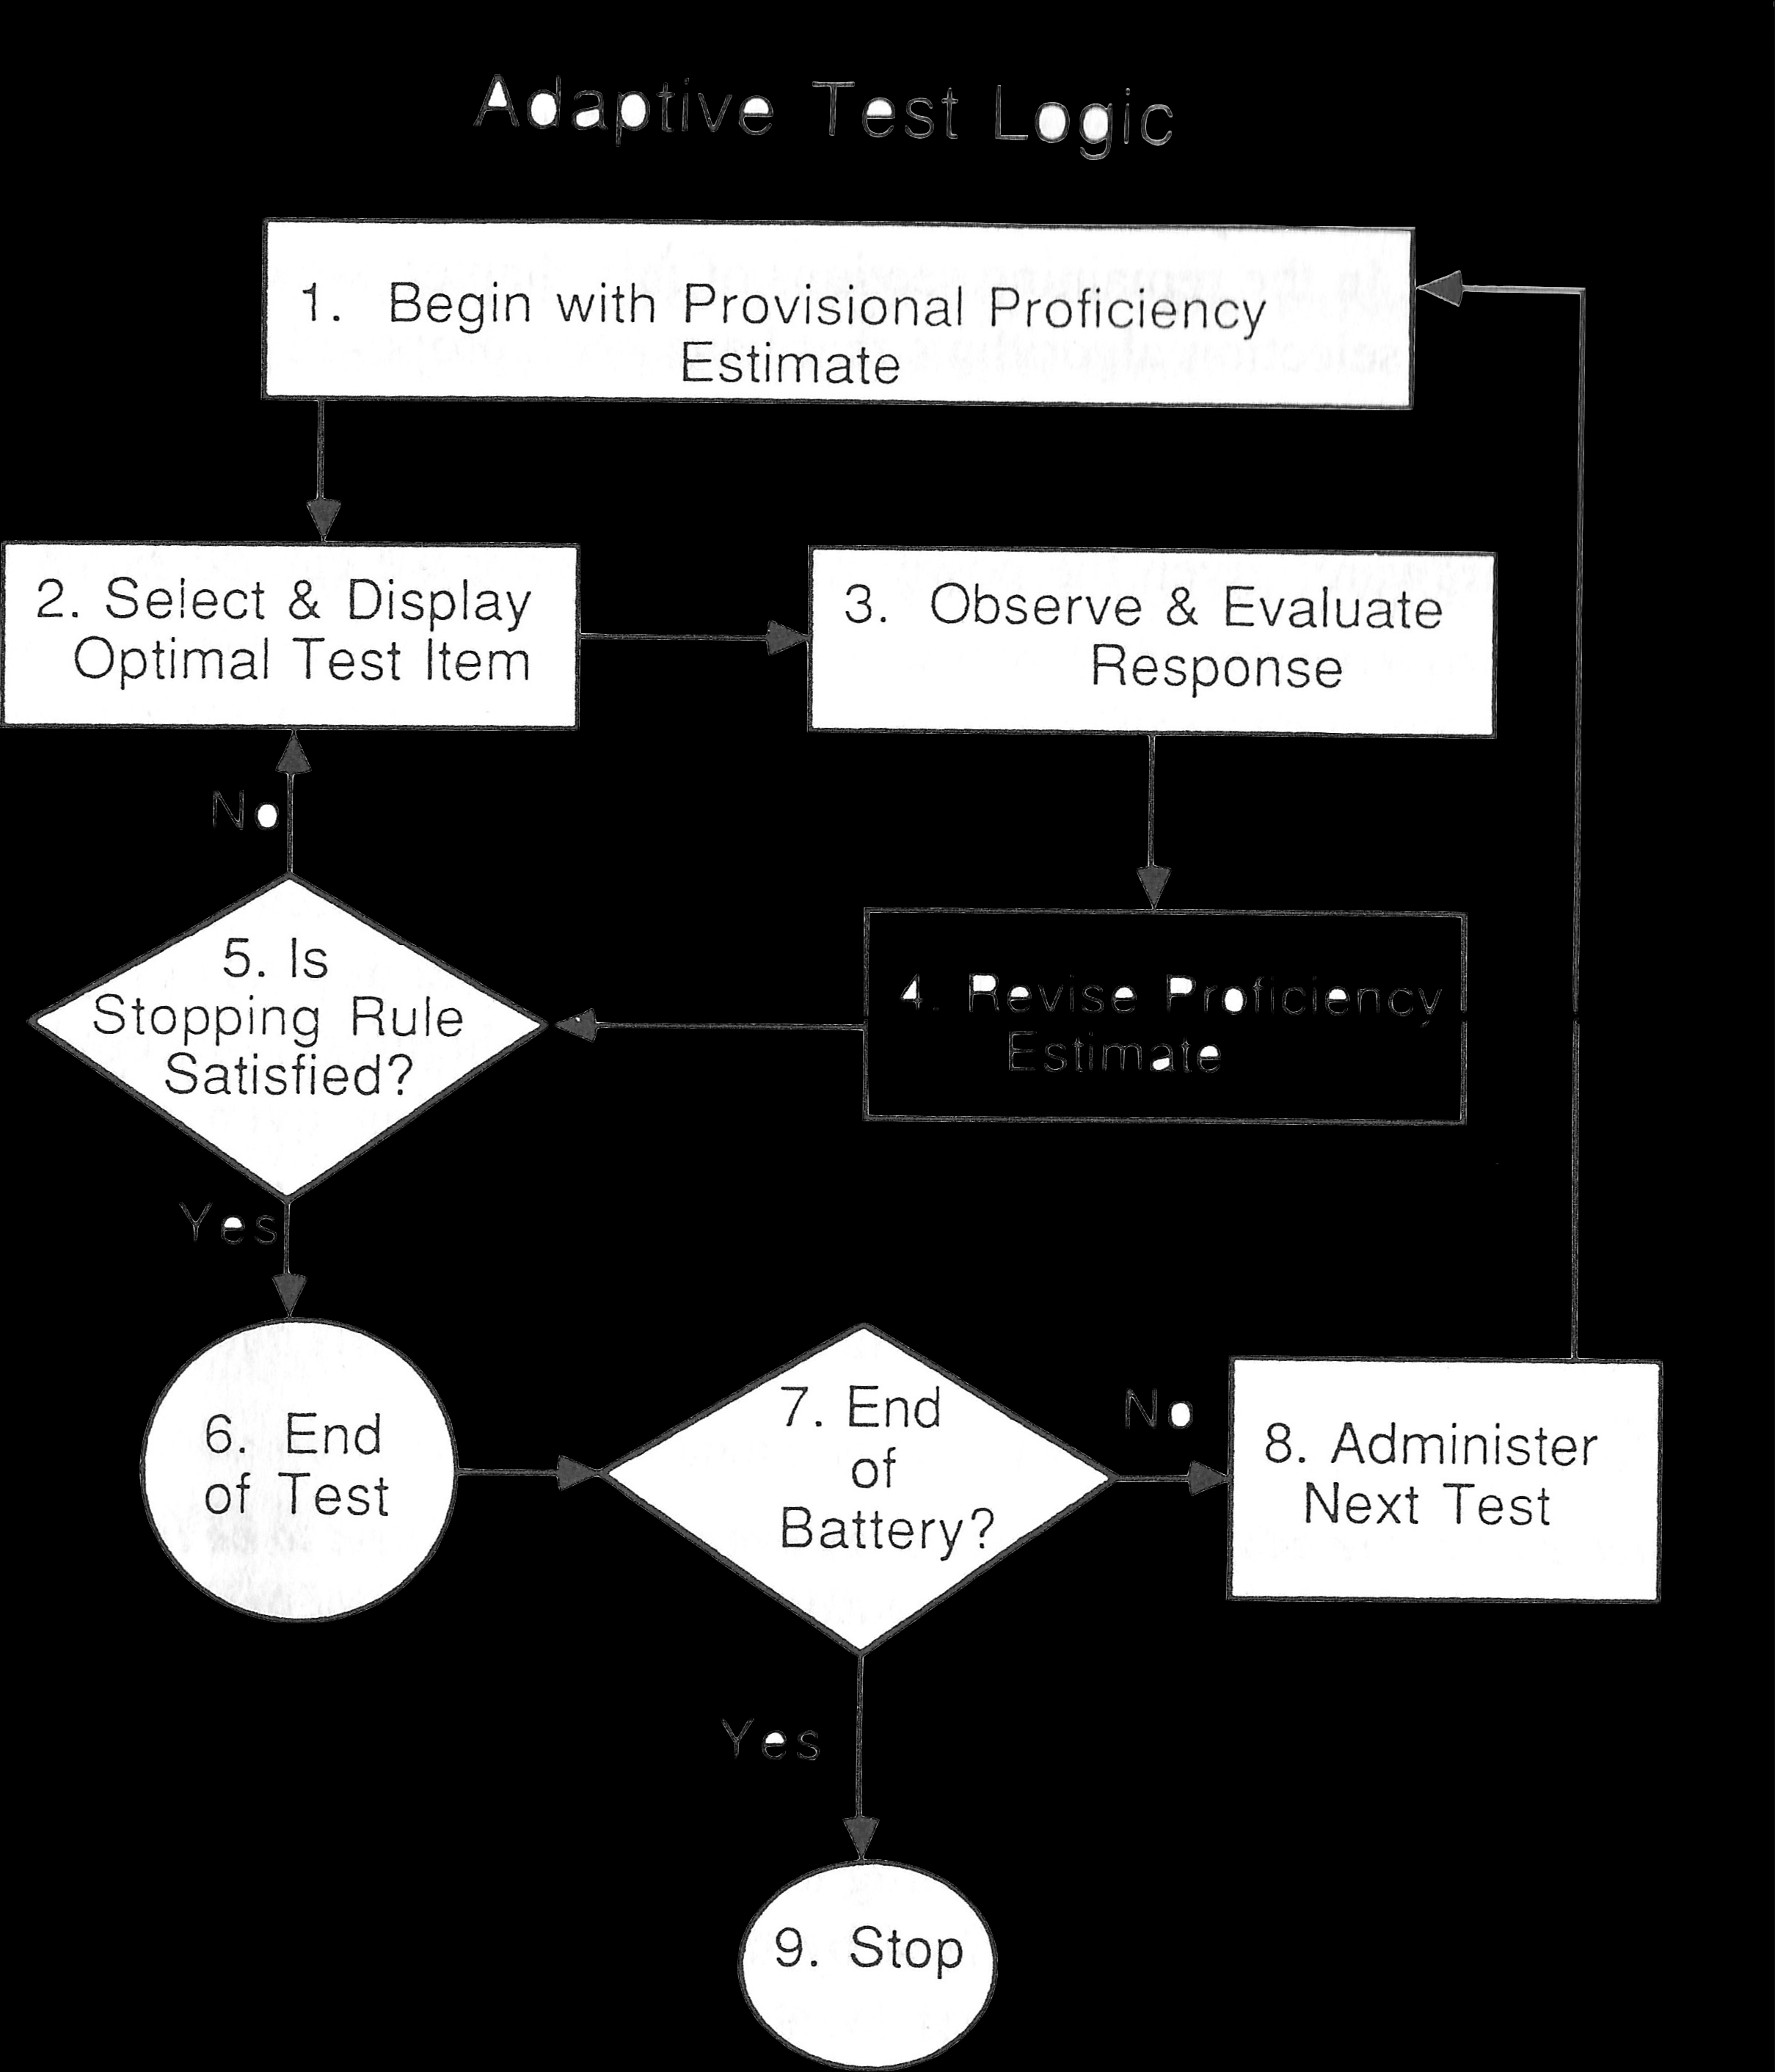
\includegraphics[width=1\textwidth,clip=true]{adaptative_test_logic}
	\caption{Diagrama de flujo de un \acrshort{CAT}}
	\label{fig:diagrama_flujo_CAT}
\end{figure}

Un importante salto ocurrió cuando el la década de los 90 se empezo a investigar la adaptación hipermedia (\acrshort{AH}), y más concretamente, la adaptación hipermedia educativa o \acrshort{AEH}.





In that framework, CAT allows seeing the
students as individuals, taking their own characteristics into
account. Typically, CAT systems are able to adapt the items
presented to the student depending on their former answers, often
including some kind of personalized feedback [12].



Constructing quality test with e-valUAM

Technology-Enhanced Learning (TEL) has a growing presence in educational institutions by making use of Computer-Aided Learning (CAL): a keynote practice where teachers and students are assisted by computers in their teaching/learning processes. Under this perspective, the assessment process is one of those issues that can get profit from the use of these practices. Moreover, completely on-line learning environments, like the emergent trends in Massive Open Online Courses (MOOCs) [1], demonstrate the importance of using CAL environments.

We can find in the literature several examples of assessment tools for some specific learning domains that can give useful and interactive advices to the students [3] [4] [5] [6]. In the context of providing feedback and advice to the students for widespread domains, Computer Adaptive Testing (CAT) provides advantages apart from an instantaneous scoring [7]. 



%
% Diseño
%
\chapter{Diseño\label{sec:disenho}}

TODO: Diseño del proyecto

%
% Desarrollo
%
\chapter{Desarrollo\label{sec:desarrollo}}

TODO: Desarrollo del proyecto

%
% Resultados
%
\chapter{Resultados\label{sec:resultados}}

TODO: Pruebas y resultados

%
% Conclusiones
%
\chapter{Conclusiones\label{sec:conclusiones}}

A modo de conclusión, a continuación se presentan los \textbf{logros más relevantes} que ha alcanzado el proyecto expuesto a lo largo de todo el documento, con los que se logran satisfacer todos los objetivos que se recogieron en la introducción:

\begin{itemize}
	\item Se ha diseñado un \textbf{sistema adaptativo} inspirado en \textit{Computerized Adaptive Testing} y la \textit{Adaptive Educational Hypermedia} que, utilizando información de modelos de usuarios, de dominio y de adaptación, permite crear cuestionarios personalizados que profesores y alumnos pueden utilizar para medir su rendimiento académico recibiendo de forma instantánea retroalimentación.
	\item Se han desarrollado las herramientas necesarias para que los profesores puedan crear las baterías de preguntas a través de una interfaz online que les abstrae de los modelos subyacentes logrando así que pueda ser utilizada por \textbf{usuarios sin conocimientos informáticos} avanzados.
	\item Se ha diseñado un sistema capaz de trabajar con \textbf{ficheros multimedia} que ofrecen más posibilidades a los profesores a la hora de crear las preguntas. Así mismo, se ha diseñado una base de datos que ha logrado almacenar toda la información sobre el uso, permitiendo análisis posteriores que han llevado a la creación de nuevos modelos y publicaciones científicas.
	\item Se han implementado mecanismos de \textbf{análisis automático} de resultados que permiten detectar a los profesores preguntas defectuosas de forma instantánea para que puedan corregirlas o eliminarlas, simplificando una tarea muy costosa.
	\item Se han construido \textbf{dos prototipos} incrementales y funcionales durante dos años académicos en los cuales han demostrado su flexibilidad, al haber sido probado en ellos varios modelos de adaptación sin que ello haya significado remodelaciones en el resto de módulos.
	\item Ambos prototipos han sido utilizados con éxito en\textbf{ dos entornos reales}, en dos disciplinas distintas y con más de 100 alumnos, habiendo situaciones donde 50 alumnos han utilizado en paralelo el sistema sin que el rendimiento bajara.
\end{itemize}

Por otra parte, aunque todos los objetivos se han cumplido, algunos, como el relativo al análisis de los resultados, podrían beneficiarse de más desarrollo. Así mismo, a lo largo del desarrollo del proyecto han ido surgiendo ideas y propuestas de mejoras del sistema y con todo ello se ha elaborado una lista de retos que desean abordarse en un futuro cercano:

\begin{itemize}
	\item Añadir \textbf{más análisis de resultados}, como remarcar preguntas que tienen un tiempo de respuesta más alto o crear informes con la evolución de cada alumno a lo largo del año o el conjunto agrado de toda la clase. Así mismo, también se desea añadir una biblioteca de gráficos en Javascript (como D3.js) para \textbf{mejorar la visualización} de todos los análisis.
	\item Permitir que se puedan crear \textbf{nuevos tipos de pregunta}, como preguntas de respuesta abierta o preguntas generadas en función a un código especificado por el profesor.
	\item Dar la opción a los profesores de \textbf{elegir qué modelo} de adaptación desean utilizar entre todos los desarrollados.
	\item \textbf{Ampliar} las opciones que ofrecen las herramientas de creación y gestión de materias, preguntas y cuestionarios que tienen accesibles los profesores.
	\item Dedicar esfuerzos en la \textbf{interacción persona-ordenador}. Para ello, se pretende recolectar información sistemática mediante cuestionarios sobre la experiencia de uso a los alumnos que ya lo han probado para solucionar las deficiencias que puedan existir y luego centrar los esfuerzos a hacer que el sistema sea \textbf{accesible} para usuarios con diversidad funcional.
	\item Facilitar las \textbf{tareas de administración} mediante una interfaz web.
\end{itemize}
 

%
% Página en blanco
%
\cleardoublepage

%
% Bibliografía
%
\bibliography{src/bibliografia}
\addcontentsline{toc}{chapter}{Bibliografía}

% No expandir elementos para llenar toda la página
\raggedbottom

%
% Apéndices
%
\appendix
\cleardoublepage
\addappheadtotoc
\appendixpage

%
% TODO: Apéndices del TFG
%
%\chapter{Análisis de requisito ampliado\label{apen:analisis de requisitos}}

\begin{rnf0}
	\item Accesibilidad
	\begin{rnf0*}
		\item El sistema debe cumplir con el estándar \acrshort{WCAG} 2.0 en un nivel A.
	\end{rnf0*}
\end{rnf0}

\chapter{Clasificación de las preguntas en niveles. Motivación y metodología\label{apend:preguntas en niveles}}

\chapter{¿Cómo se evaluan los cuestionarios?\label{apen:como se ponen las notas}}


\chapter{Estructura del proyecto\label{apen:estructura proyecto}}

\chapter{Código más relevante\label{apen:codigo}}


%
%\chapter{Ejemplos de bloques y comandos útiles en LaTeX\label{sec:ejemplos}}
%\section{Ejemplo de sección}
%
%
% Breve guía de comandos útiles para la memoria
%
%
% Citar una referencia
%La DARPA creo el protocolo de Internet \cite{ipv4sta}.
%
% Citar un elemento del glosario
%Citamos el acrónimo \gls{FPGA}.
%
% Citar un elemento del glosario (primera letra en may´usculas)
%\Gls{bitstream} es una secuencia de bits.
%
% Insertar una imagen con pie de página
%\begin{figure}[htp!]
%  \centering
%  
\includegraphics[width=0.75\textwidth,clip=true]{Logo_UAM}
%  \caption{Logo de la Universidad Autónoma de madrid.}
%  \label{fig:logo_uam}
%\end{figure} 
%
% Referenciar una etiqueta (label)
%La figura~\ref{fig:logo_uam} se utiliza en la portada.
%
% Nueva página
%\clearpage
%
% Añadir código fuente sin líneas
%\begin{lstlisting}[label=algoritmo:quicksort,language=C,frame=single,caption=Algoritmo de ordenación Quicksort]
%#include <stdio.h>
% 
%void quick_sort (int *a, int n) {
%    int i, j, p, t;
%    if (n < 2)
%        return;
%    p = a[n / 2];
%    for (i = 0, j = n - 1;; i++, j--) {
%        while (a[i] < p)
%            i++;
%        while (p < a[j])
%            j--;
%        if (i >= j)
%            break;
%        t = a[i];
%        a[i] = a[j];
%        a[j] = t;
%    }
%    quick_sort(a, i);
%    quick_sort(a + i, n - i);
%}
%\end{lstlisting}
%
% Bloque de código inseparable
%\begin{code}
%#include <stdio.h>
% 
%void quick_sort (int *a, int n) {
%    int i, j, p, t;
%    if (n < 2)
%        return;
%    p = a[n / 2];
%    for (i = 0, j = n - 1;; i++, j--) {
%        while (a[i] < p)
%            i++;
%        while (p < a[j])
%            j--;
%        if (i >= j)
%            break;
%        t = a[i];
%        a[i] = a[j];
%        a[j] = t;
%    }
%    quick_sort(a, i);
%    quick_sort(a + i, n - i);
%}
%\end{code}
%
% Fórmula dentro de una línea de texto
%La ecuación de Euler ($e^{ \pm i\theta } = \cos \theta \pm i\sin \theta$) es citada frecuentemente como un ejemplo de belleza matemática.
%
% Fórmula independiente
%\begin{equation}\label{eq:pythagoras}
%a^2 + b^2 = c^2
%\end{equation}


% Fin del documento
\end{document}
